The gaze inference component of our approach analyzes the input body motion and virtual scene and constructs a model of gaze movements as a sequence of gaze instances. Each gaze instance is a tuple $G = (f_s, f_x, f_e, T, \alpha_{H}, \alpha_{T})$, where $f_s$, $f_x$, and $f_e$ are gaze shift start frame, fixation start frame, and fixation end frame, respectively, and $T$ is the gaze target. $\alpha_{H}$ and $\alpha_{T}$ are the head and  torso \emph{alignment} parameters, which specify head and torso orientation relative to the target and serve as inputs into the gaze shift model (Section~\ref{sec:GazeShiftModel}). These parameters enable facile control over head and torso pose during gaze editing.

Gaze inference begins with a signal analysis of the body motion to detect individual gaze instances and infer their timings, $f_s$, $f_x$, and $f_e$. The inferred sequence may contain gaps, during which no directed gaze is applied to the character---we refer to such gaps as \emph{unconstrained gaze}. Next, we analyze the character's view of the scene at the end of each gaze shift and infer the most probable target $T$. Finally, we compute the alignment parameter values, $\alpha_{H}$ and $\alpha_{T}$, from the head and torso poses at the end of each gaze shift.

\subsection{Gaze Instance Inference}
\label{sec:GazeTimingInference}

Human gaze shifts follow a particular kinematic pattern. The eyes, head, and torso accelerate toward the gaze target, reach their peak velocities at the midpoint of the gaze shift, and decelerate as they align with the target, at which point the fixation begins. We detect gaze shifts by searching for this pattern in the body motion using a three-step approach. First, we search for clusters of maxima in angular acceleration signals of the head and torso joints, which correspond to significant gaze events (gaze shift beginnings and ends).~\citet{coleman2008staggered} used a similar method for key pose extraction. Each pair of adjacent gaze events defines the boundaries of a motion interval, which can be either a gaze shift or a fixation. In the second step, we classify the motion intervals into gaze shifts and fixations. Third, for each adjacent gaze shift-fixation pair, we generate a gaze instance.

\begin{figure}
\centering
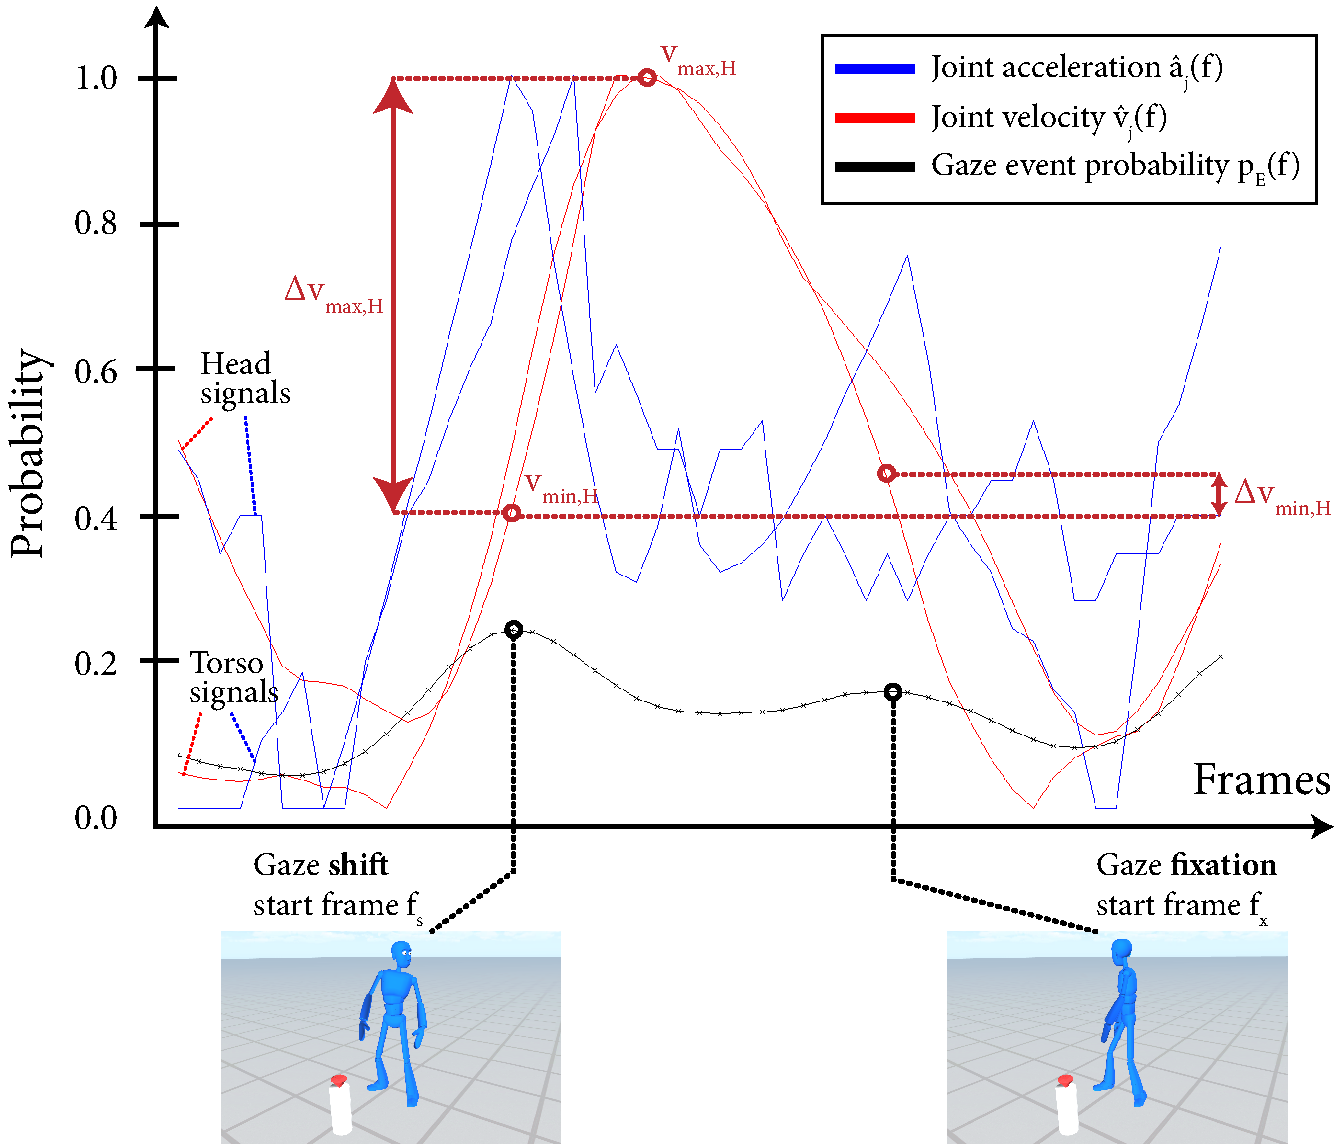
\includegraphics[width=1\textwidth]{gazeauthoring/Figures/GazeInstanceInference.pdf}
\caption{Gaze shift detection through analysis of acceleration and velocity signals of the head and torso. We first aggregate the normalized joint accelerations $\hat{a}_j(f)$ into a global probability signal $p_E(f)$. Adjacent local maxima in $p_E(f)$ define the boundaries of a motion interval. We determine that the interval is a gaze shift from its high peak velocity, $v_{\mathrm{max},j}$. Velocity signals in the graph were normalized for easier viewing, whereas inference is performed on unnormalized velocities.}
\label{fig:GazeInstanceInference}
\end{figure}

\subsubsection{Gaze Event Discovery}

We discover gaze events by analyzing joint accelerations in the motion (Figure~\ref{fig:GazeInstanceInference}). Let $a_j(f)$ be the angular acceleration signal of the joint $j$, defined across the motion's frame range ($f \in [0, L\rangle$, where $L$ is motion length in frames). We normalize the acceleration signals to the 0-1 range: $\hat{a}_j(f) = a_j(f) / \mathop{max}(a_j(f))$. We use the normalized acceleration signals of the root, torso, and head joints as local evidence measures indicating probability of significant gaze events (i.e., gaze shift beginning or ending). We compute the global probability of a gaze event as a weighted sum of normalized acceleration signals:
%
\begin{align} \label{eq:GazeEventProbability}
p_E(f) = \frac{\sum_{j \in J} w_j \hat{a}_j(f)}{\sum_j w_j}
\end{align}
%
where $J$ is the set of joints, consisting of the root, torso, and head joints. Weights $w_j$ define each joint's influence on the global probability. We heuristically define a joint's weight to be greater the closer it is to the eyes, i.e., the head contributes more to the global probability than the torso or root. This choice is based on findings showing the importance of head movements for the execution and perception of human gaze~\citep{hietanen1999does}. We calculate joint weights as follows:
%
\begin{align} \label{eq:GazeJointWeight}
w_j(f) = \frac{1}{1 + l_j}
\end{align}
%
where $l_j$ is the distance between joint $j$ and the eyes, measured as the cumulative length of the segments between them.

Local maxima in $p_E$ correspond to the beginnings and endings of gaze shifts. Since acceleration signals are likely to be noisy and contain a large number of spurious maxima, a bilateral filter is applied to $p_E$ to smooth out the spurious maxima while preserving those that are kinematically significant. We set the filter's range parameter $\sigma_r$ to 0.5 and spatial parameter $\sigma_s$ to 3. The filtered probability signal is then searched for local maxima. Each pair of adjacent maxima defines a motion interval $I_k = (f_{s,k}, f_{e,k})$, which could either be a gaze shift or a fixation.

\subsubsection{Motion Interval Classification}

To determine if a motion interval $I_k$ is a gaze shift, we use the fact that gaze shifts are characterized by peaks in joint velocity (Figure~\ref{fig:GazeInstanceInference}) and we construct another probabilistic measure. Let $v_j(f)$ be the angular velocity signal of joint $j$. We define $v_{s,j}^k$ and $v_{e,j}^k$ to be joint velocities at the boundaries of the interval $I_k$. Furthermore, let $v_{\mathrm{max},j}^k$ and $v_{\mathrm{min},j}^k$ be the maximum and minimum joint velocity over the interval $I_k$. Then we define maximum and minimum velocity differences as $\Delta v_{\mathrm{max},j}^k = v_{\mathrm{max},j}^k - \mathop{min} (v_{s,j}^k, v_{e,j}^k)$ and $\Delta v_{\mathrm{min},j}^k = \mathop{max} (v_{s,j}^k, v_{e,j}^k) - v_{\mathrm{min},j}^k$. Finally, we define the ratio of these quantities as follows:
%
\begin{align} \label{eq:GazeShiftRatio}
r_j^k =
\begin{cases}
0 & \text{if} \Delta v_{\mathrm{max},j}^k \leq 0 \\
\frac{\Delta v_{\mathrm{max},j}^k}{\Delta v_{\mathrm{min},j}^k} & \text{otherwise}
\end{cases}
\end{align}
%
The ratio $r_j^k$ increases with peak velocity relative to the velocities at interval boundaries, indicating a gaze shift at the interval. A logistic function then maps the ratio to a probability value in the 0--1 range:
%
\begin{align} \label{eq:GazeShiftProbability}
p_{S,j}^k = \frac{2}{1 + \mathop{exp}(-r_j^k)} - 1
\end{align}
%
Finally, we compute the gaze shift probability as a weighted sum of per-joint probabilities:
%
\begin{align} \label{eq:GazeShiftGlobalProbability}
p_S^k = \frac{\sum_{j \in J} w_j p_{S,j}^k}{\sum_j w_j}
\end{align}
%
where $w_j$ are the joint weights defined previously.

We classify the interval $I_k$ as a gaze shift if $p_S^k > P_{S,\mathrm{min}}$ (where $P_{S,\mathrm{min}}$ is a probability threshold set to 0.6) and as a fixation otherwise. Adjacent intervals that are classified as fixations get aggregated into a single fixation. We end up with a sequence of gaze shift-fixation pairs, from which we generate the sequence of gaze instances.

\subsubsection{Gaze Instance Generation}

For each gaze shift-fixation pair $(I_k, I_l)$, we generate a gaze instance $G = (f_s, f_x, f_e)$, such that the gaze shift starts at $f_s = f_{s,k}$, while the fixation starts at $f_x = f_{s,l}$ and ends at $f_e = \mathop{min}(f_{e,l}, f_{s,l} + L_\mathrm{max} - 1)$. Note that the fixation may not be longer than $L_\mathrm{max}$ (set to 1 second by default)--this is to prevent gaze from becoming ``stuck'' on a target for long periods of time.

Gaze shift probability threshold $P_\mathrm{min}$ is a useful parameter for controlling the density of gaze shifts found by the inference. Lowering the parameter to 0.5 results in subtle head and body movements being detected as gaze shifts and yields a more expressive behavior, albeit one that may be more challenging to edit---this setting was used for the ChatWithFriend example (~\ref{fig:GazeEditResults}, 5), which contains a lot of conversational gaze aversions. On the other hand, at parameter values above 0.6 only the most obvious gaze shifts are picked up, yielding a sparse gaze behavior that can be enriched further through manual editing.

\subsection{Gaze Target Inference}
\label{sec:GazeTargetInference}

In the preceding step, we inferred all the gaze instances and their timings. Next, for each gaze instance we infer its target in the scene. We assume there exists at least a simplified 3D model of the scene containing the key characters and objects, like those used for pre-visualization. The result of gaze target inference is a sequence of gaze instances with associated targets. Gaze targets are handles in the scene attached to objects and other characters, which the animator can move around to change where the character is looking.

Our gaze inference method is based on three heuristics. First, the character is more likely to be looking at a point that lies along the movement direction of its head. If the character turns right, it is unlikely that the target lies to the left, up, or down. Second, the character is more likely to look at objects and characters that are \emph{important} to the story or task. For instance, in a scene where the character steals a gem, the gem is a likely gaze target. We let the animator manually label scene objects as important. Finally, the character is more likely to gaze at objects just before touching or picking them up~\citep{johansson2001eyehead}. Assuming hand contacts are annotated in the body motion, we can easily determine when the character is about to handle an object.

We use a probabilistic approach for gaze target inference. Recall the gaze instance specification from the preceding step: $G = (f_s, f_x, f_e)$. The gaze fixation start time, $f_x$, is when the character's eyes are aligned with the target; therefore, the target must be within the character's view. We compute a probability distribution, $p_T(\mathbf{x})$, over the 2D projection space representing the character's view of the scene at the frame $f_x$. Here $\mathbf{x}$ denotes a point in the 2D projection space. For every point in the character's view, $p_T(\mathbf{x})$ gives us the probability that the character is gazing at it. We find the gaze target $T$ at the global maximum of $p_T$.

We model $p_T(\mathbf{x})$ as a weighted sum of three probability terms, each implementing one principle of gaze target inference:
%
\begin{align} \label{eq:GazeTargetGlobalProbability}
p_T = \frac{w_d p_d + w_i p_i + w_h p_h}{w_d + w_i + w_h}
\end{align}
%
$p_d(\mathbf{x})$ is the directional term, which assigns higher probabilities to points lying along the direction of head movement. $p_i(\mathbf{x})$ is the importance term and is non-zero at points corresponding to objects and characters labeled as important. $p_h$ is the hand contact term, which is non-zero for objects that are about to be handled by the character. These terms contribute to the final probability, $p_T$, in proportion to their weights, $w_d$, $w_i$, and $w_h$. We empirically find that the best inference results are obtained by setting these weights to 0.6, 0.15, and 0.25, respectively. Given the final probability $p_T$, we obtain the gaze target $T$ at the global maximum of $p_T$: $\mathbf{x}_T = \mathop{argmax}_{\mathbf{x}} p_T(\mathbf{x})$.

Figure~\ref{fig:GazeTargetInference} shows an example scene view with the associated probability distributions and gaze target location indicated. In the remainder of this section, we provide more detail about the computation of individual probability terms.

\begin{figure*}
\centering
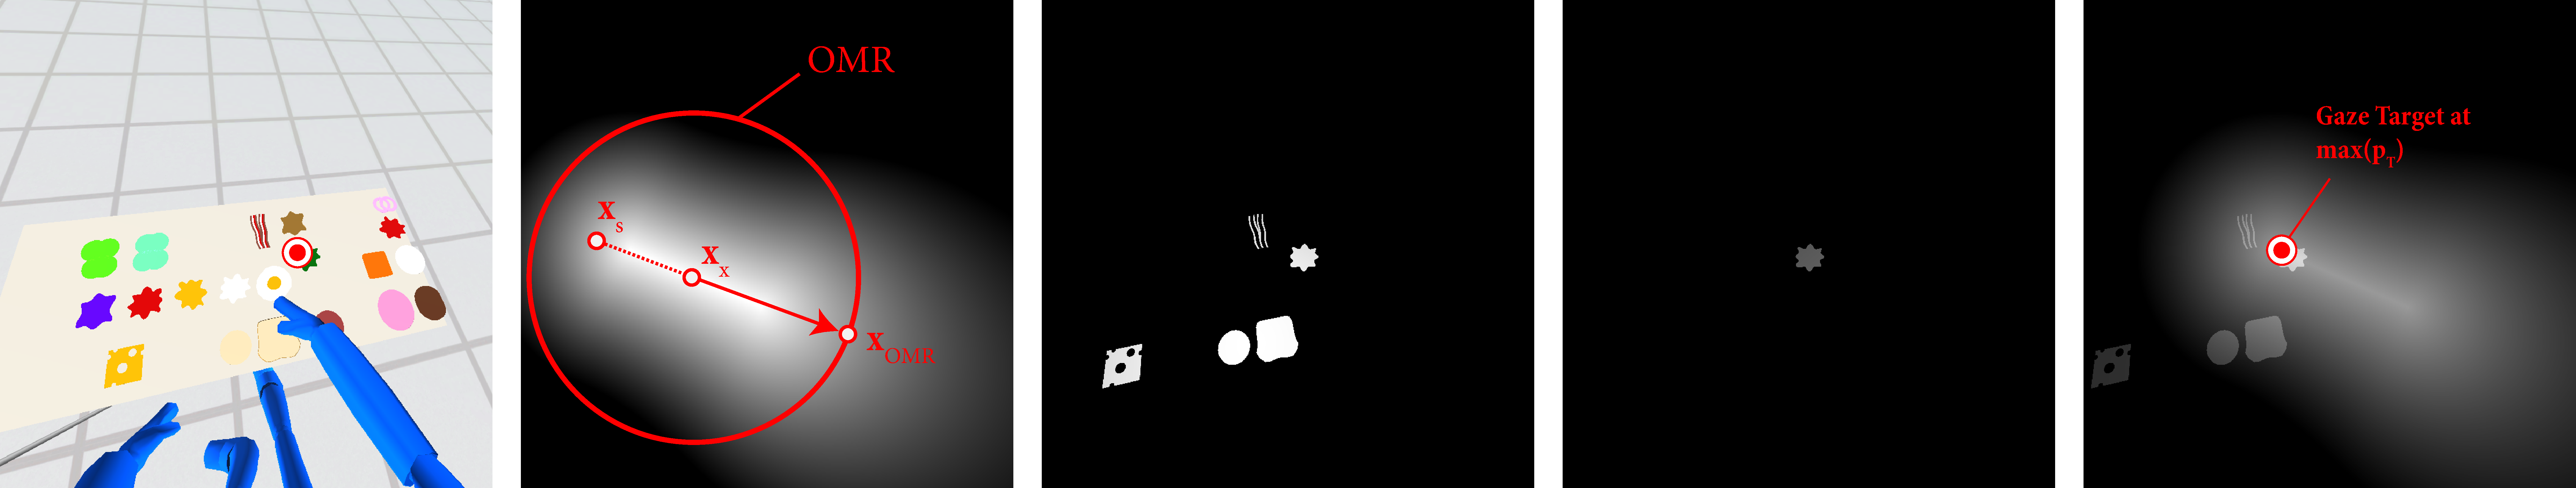
\includegraphics[width=1\textwidth]{gazeauthoring/Figures/GazeTargetInference.pdf}
\caption{We infer the gaze target by analyzing the character's scene view at the end of the gaze shift (1). The gaze target is more likely to be located along the head movement direction (directional term, 2), on an object labeled as important (importance term, 3), or on an object that is about to be touched or picked up (hand-contact term, 4). We average these probability terms and find the target at the global maximum (5).}
\label{fig:GazeTargetInference}
\end{figure*}

\subsubsection{Directional term}

The computation of the directional term, $p_d(\mathbf{x})$, is based on the following idea. When the character shifts its gaze, its head traces a path in the projection space beginning at $\mathbf{x}_s$ and ending at $\mathbf{x}_x$ (Figure~\ref{fig:GazeTargetInference}-2). If the character always gazed straight on, then $p_d(\mathbf{x})$ would be highest at $\mathbf{x}_x$. However, the character is as likely to be looking at something out of the corner of the eye, so the eyes may ``overshoot'' $\mathbf{x}_x$ and line up with a point further along the movement path. Therefore, from the path $(\mathbf{x}_s, \mathbf{x}_x)$ we extrapolate a path extending to the point $\mathbf{x}_{\mathrm{OMR}}$, which lies on the edge of the eyes' motor range (OMR), beyond which the eyes cannot move (Figure~\ref{fig:GazeTargetInference}b). $p_d(\mathbf{x})$ has the maximum value of 1 along the path $(\mathbf{x}_x, \mathbf{x}_{\mathrm{OMR}})$ and linearly falls off to zero with distance from the path.

We compute the probability fall-off as follows. Let $\mathbf{v}$ be the vector pointing from the eye centroid to the current point $\mathbf{x}$ in the projection space. Let $\mathbf{x}'$ be the projection of $\mathbf{x}$ onto the line $(\mathbf{x}_{\mathrm{OMR}}$ and $\mathbf{v}'$ the vector from the eye centroid to $\mathbf{x}'$. We denote $\phi$ the angle between vectors $\mathbf{v}$ and $\mathbf{v}'$, and we compute the probability at $\mathbf{x}$:
%
\begin{align} \label{eq:GazeDirectionProbability}
p_d(\mathbf{x}) =
\begin{cases}
1 - \frac{\phi}{OMR} & \text{iff } \phi \leq OMR \\
0 & \text{otherwise}
\end{cases}
\end{align}
%
where $OMR$ is between $45\deg$ and $55\deg$ for humans.

Note that we do not set $p_d$ to zero everywhere outside the OMR region. Due to variability in human OMR and differences between the capture environment and the virtual scene, the gaze target may actually lie outside the character's OMR. By allowing non-zero probability beyond that range, we allow our algorithm to pick up the gaze target even in such cases.

\subsubsection{Importance term}

he importance term, $p_i(\mathbf{x})$, increases the probability of placing gaze target handles on important objects and characters (Figure~\ref{fig:GazeTargetInference}-3). Let $\Omega_i$ be the (possibly discontiguous) region in the projection space occupied by projections of all the visible, important objects. The importance term is computed as:
%
\begin{align} \label{eq:GazeImportanceProbability}
p_i(\mathbf{x}) =
\begin{cases}
\mid \mathbf{v} \cdot \mathbf{n} \mid & \text{iff } \mathbf{x} \in \Omega_i  \\
0 & \text{otherwise}
\end{cases}
\end{align}
%
$\mathbf{v}$ is the vector from the eye centroid to the current projection point $\mathbf{x}$ and $\mathbf{n}$ is the object's surface normal at that point. We use the dot product to increase the probability of placing gaze target handles on the more salient parts of the object's surface rather than along the silhouette.

\subsubsection{Hand contact term}

The hand contact term, $p_h$, increases the probability of placing gaze target handles on an object that the character is about to pick up or touch. As shown in studies of human eye-hand coordination~\cite{johansson2001eyehead}, gaze toward the object is most likely to occur 1 second before hand contact, though it may begin 3 seconds before and end up to 0.6 seconds after. We use this rule to compute our probability term. If $t_x$ is the current time in the motion (corresponding to fixation start frame $f_x$) and $t_h$ is the start time of a hand contact with an object (obtained from hand contact annotations), then probability of gaze toward that object is:
%
\begin{align} \label{eq:GazeHandContactProbabilityTime}
p_{h,0} =
\begin{cases}
0 & t_x < t_h - 3 \\
\frac{t_x - t_h + 3}{2} & t_x \geq t_h - 3 \wedge t_x < t_h - 1 \\
\frac{t_x - t_h + 1}{1.6} & t_x \geq t_h - 1 \wedge t_x < t_h + 0.6 \\
0 & t_x \geq t_h + 0.6
\end{cases}
\end{align}
%
We define $\Omega_h$ to be the region of the projection space occupied by the handled object. The hand contact probability term (Figure~\ref{fig:GazeTargetInference}d) is computed as follows:
%
\begin{align} \label{eq:GazeHandContactProbability}
p_h(\mathbf{x}) =
\begin{cases}
p_{h,0} \mid \mathbf{v} \cdot \mathbf{n} \mid & \text{iff } \mathbf{x} \in \Omega_i  \\
0 & \text{otherwise}
\end{cases}
\end{align}
%
This is similar to the importance term, except that maximum probability is scaled by $p_{h,0}$.

\subsubsection{Implementation}

To achieve reasonable computation time, we compute gaze target probabilities on the GPU. We render the scene in multiple passes using a wide-angle camera located at the character's eyes and pointed in the same direction as the head. On each pass, we compute one of the probability terms $p_d$, $p_i$, and $p_h$ in a shader program. We blend the terms to get the final probability $p_T$. We then retrieve the render texture containing $p_T$ and do a linear search for $\mathbf{x}_T$. Finally, we use a raycast through $\mathbf{x}_T$ to determine the gaze target's 3D position and the scene object to which it is attached.

\subsection{Computing Alignment Parameters}
\label{sec:GazeAlignmentInference}

Having inferred all the gaze instances and their targets, we also compute the values of the head and torso alignment parameters, $\alpha_{H}$ and $\alpha_{T}$. When humans shift their gaze, they may also reorient their head or torso toward the target, which affects how the gaze shift is perceived by others. For example, looking at something out of a corner of the eye signals a lower level of attention than when turning the head to face the target fully.

Our gaze synthesis approach (Section~\ref{sec:GazeSynthesis}) allows the animator to control the amount of head and torso reorientation using the alignment parameters, $\alpha_{H}$ and $\alpha_{T}$, and thus obtain a greater variety of gaze shifts. Parameter values range from 0 to 1, where 0 specifies minimal reorientation, while 1 fully aligns the head or torso with the target (Figure~\ref{fig:GazeShiftExamples}). During gaze inference, we compute the values of the alignment parameters that match the postures encoded in the original motion. The animator can then edit the postures by hand-editing the alignment values (Section~\ref{sec:GazeEditing}).

Knowing the timing and target of each gaze shift, we can analytically estimate the head and torso alignment values by effectively reversing the procedure for gaze shift target directions computation, depicted in Figure~\ref{fig:GazeShiftTargetRot}. Let $f_s$ be the start frame and $f_x$ the end frame of the gaze shift. The torso rotates from the orientation $\mathbf{q}_T^s$ and stops at $\mathbf{q}_T^x$. We set the character to the start pose and compute $\mathbf{q}_{\mathrm{full},T}$, which is the orientation which would fully align the torso joint with the target (corresponding to $\alpha_T = 1$), and $\mathbf{q}_{\mathrm{min},T}$, which is the minimal torso orientation (corresponding to $\alpha_{T} = 0$). Next, we project $\mathbf{q}_{T}^x$ onto the arc defined by orientations $\mathbf{q}_{T}^s$ and $\mathbf{q}_{\mathrm{full},T}$---we denote this projected orientation $\mathbf{q}_{T,\mathrm{proj}}$. Finally, we compute $\alpha_T$ as:
%
\begin{align} \label{eq:GazeAlignmentInference}
\alpha_T = \frac{\angle(\mathbf{q}_{T,\mathrm{proj}}, \mathbf{q}_{\mathrm{min},T})}{\angle(\mathbf{q}_{\mathrm{full},T}, \mathbf{q}_{\mathrm{min},T})}
\end{align}
%
The procedure for computing $\alpha_{H}$ is analogous.

\subsection{Evaluation}
\label{sec:GazeInferenceEvaluation}

The purpose of gaze inference is to infer an editable gaze behavior that fits the character's body motion and scene. This involves (1) detecting key gaze shifts in the original motion and (2) inferring gaze target handles on important objects. We have evaluated the effectiveness of the gaze inference component on both criteria, while using motion capture, eye tracking, and human annotation data as ground-truth.

\subsubsection{Data Collection}

We acquired ground-truth body motion and eye tracking data using a Motion Analysis optical motion capture system and SMI Eye Tracking Glasses. We recorded nine scenes, in which the actor engaged in activities with rich gaze behaviors: environment interactions, locomotion, two-person conversation, and so on. The cumulative length of all the motions was 6:46 minutes. Next, we had two human coders annotate \emph{gaze shifts} and \emph{important gaze targets} in each scene. For gaze shift annotations, the coders were instructed to visually analyze body motion kinematics and mark gaze shift start and end times. For gaze target annotations, we selected five scenes that involved extensive gaze toward important objects, with a total length of 4:57 minutes. From the eye tracker video, we extracted representative image frames for each fixation detected by the eye tracker. Finally, we instructed the coders to annotate the gaze target in each image. For example, for the StealGem scene, any frame showing gaze toward the gem object was marked ``Gem.''

\subsubsection{Results: Gaze Instances}

Out of the total motion dataset, 2:30 minutes were annotated by both coders, allowing us to compute intercoder agreement. We first identified pairs of overlapping gaze shift annotations in both datasets. We found that 81\% of the gaze shifts in the first dataset had a match in the second dataset, and 90\% of the gaze shifts in the second dataset had a match in the first dataset. Next, we measured correlation of gaze shift start times and end times between the two datasets using Fisher's formula for intraclass correlation~\cite{fisher1925statistical}. We obtained $r = 1.00$ for both start and end times, indicating very high correlation between the coders' estimates of gaze shift timings.

We used a similar approach to measure the accuracy of gaze instance inference. First, we identified pairs of overlapping gaze shifts in the inference output and ground-truth annotations. Next, we computed the \emph{sensitivity} of gaze instance inference, which is the percentage of ground-truth gaze shifts that had a match in the inference output. This measure is significant because it tells us how effective the inference method is at picking up key gaze shifts. Finally, for the pairs of overlapping gaze shifts, we computed Fisher's r as a measure of correlation of their start times ($t_s$) and end times ($t_e$), respectively. Table~\ref{tab:GazeShiftInferenceResults} shows the evaluation results for all nine scenes.

\begin{table}
\small
\centering
\def\arraystretch{1.5}
\begin{tabular}{lrrr}
\hline
\textbf{Scene} & \textbf{Sensitivity} & $r(t_s)$ & $r(t_e)$ \\
\hline
WindowWashing & 86\% & 1.00 & 1.00 \\
WalkCones & 58\% & 0.99 & 0.99 \\
BookShelf & 84\% & 1.00 & 1.00 \\
StealDiamond & 80\% & 1.00 & 0.99 \\
WaitForBus & 97\% & 1.00 & 1.00 \\
StackBoxes & 69\% & 1.00 & 1.00 \\
MakeSandwich & 100\% & 1.00 & 1.00 \\
MakeSandwichDemo & 81\% & 1.00 & 1.00 \\
ChatWithFriend & 58\% & 1.00 & 1.00 \\
\hline
\end{tabular}
\caption{Results of gaze instance inference evaluation}
\label{tab:GazeShiftInferenceResults}
\end{table}

For the ChatWithFriend scene we found that our method achieved relatively low sensitivity. This scene depicts a character standing and conversing with another person. Most of the gaze shifts are conversational gaze aversions involving subtle head movements, which may be difficult to detect using our method.

\subsubsection{Results: Gaze Targets}

As with gaze shift annotations, we had our coders independently annotate an overlapping portion of the dataset that was comprised of three scenes with a total length of 2:32 minutes. We calculated Cohen's $\kappa$ as the measure of inter-coder agreement; $\kappa$ ranged from 0.93 to 1.00, indicating very high agreement.

Next, we evaluated the accuracy of gaze target inference as follows. Our analysis included only gaze instances toward important scene objects and characters. For each gaze instance in the inference output, we searched for overlapping fixations in the ground-truth data. If there was at least one fixation where the target label matched the inferred target for that instance, we counted the instance as correct. The percentage of correctly inferred instances served as inference accuracy. Accuracies for the five scenes were as follows: BookShelf (63\%), StealDiamond (100\%), StackBoxes (50\%), ChatWithFriend (83\%), and MakeSandwichDemo (82\%). Low accuracy of the StackBoxes scene may be due to errors in ground-truth data, as the scene involved downward glances toward boxes carried by the actor, which may have lain beyond the field of view of the eye tracker camera.
